\documentclass{article} % For LaTeX2e
\usepackage{nips13submit_e,times}
\usepackage{hyperref}
\usepackage{url}
\usepackage{graphicx}
\usepackage{fancyvrb}
\usepackage{amsmath}
\usepackage{amssymb}
\usepackage{mathtools}
\usepackage{caption}
\usepackage{subcaption}
%\documentstyle[nips13submit_09,times,art10]{article} % For LaTeX 2.09


\title{Identifying features of stock market patterns}


\author{
Jimmy\\
University of Billion Chinese\\
Vancouver, BC \\
\texttt{jimmec@gmail.com} \\
\And
Ricky\\
University of Building Construction\\
Vancouver, BC \\
\texttt{rickychen92@gmail.com} \\
}

% The \author macro works with any number of authors. There are two commands
% used to separate the names and addresses of multiple authors: \And and \AND.
%
% Using \And between authors leaves it to \LaTeX{} to determine where to break
% the lines. Using \AND forces a linebreak at that point. So, if \LaTeX{}
% puts 3 of 4 authors names on the first line, and the last on the second
% line, try using \AND instead of \And before the third author name.

\newcommand{\fix}{\marginpar{FIX}}
\newcommand{\new}{\marginpar{NEW}}

\nipsfinalcopy % Uncomment for camera-ready version

\begin{document}


\maketitle

\begin{abstract}
Technical analysis is a methodology for analyzing financial markets and forecasting future price movements. Practioners often rely on their ability to identify recurrent patterns to make predictions. In this paper we attempt to identify features of a time series that captures the patterns used in technical analysis and visually evaluate the efficacy of these features through a t-distributed Stochastic Neighbour Embedding \cite{Hinton08tsne} into a low dimensional space. The assumption is that features that truly captures technical analysis patterns will group samples with similar patterns near each other in the feature space, thus, a neighbourhood preserving map such as the t-SNE should allow visual identification of clusters of patterns even in low dimensions. In the first section, we give a breif description of technical analysis and motivations for this paper. Then, we describe the methods we use to preprocess and extract samples from raw time series. Finally, we present the results obtained under various features we tested.
\end{abstract}

\section{Introduction}
In the world of investing, there are two major schools of thought concerning the future price forecasting, fundamental analysis and technical analysis. The former relies on explicitly analyzing the financial reports and underlying market conditions such as the economic trend or the weather patterns of a growing season. In contrast, technical analysis is built on the premise that a time series plot of a security's price fully reflect all market conditions underlying said security. 

One of the predictors technical analysts look for are chart patterns in the price time series. Chart patterns generally fall under one of the 2 categories: continuation patterns and reversal patterns; as their names suggest, the former reaffirms the current direction of price movement while the ladder signals a change. While the patterns in \ref{patterns} appear to be completely arbitrary, the predictive power of these patterns can be understood in terms of the psychological aspect of financial markets. Widespread adoption of the practice in market analysis can cause patterns to become a self-fulfilling prophecy.

\begin{figure}[h]
\begin{center}
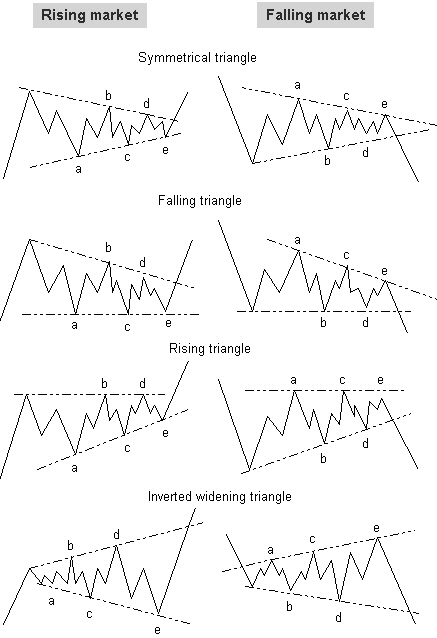
\includegraphics[width=0.7\textwidth]{chart_patterns.jpg}
\end{center}
\caption{Common technical analysis patterns \label{patterns}}
\end{figure}

However, identifying patterns come with a steep learning curve and are prone to human error for beginners. Thus, it's natural to try to frame this in a more rigorous manner. To that end, we need to develop a set of features that correctly describe the patterns so that machine learning techniques may be applied for clustering and classification. Since we have no means of obtaining labeled data, our project proposes a framework for evaluating the efficacy of features by visualizing the intrinsic clusters created by them. It then becomes feasible to manually inspect a few representative samples from each cluster to see if the group indeed reflect a textbook pattern. Our project is motivated by previous works on pattern recognition using neural networks \cite{Guo07recognizingstock}.


\section{Methodology}
\subsection{Time series segmentation}
For a time series $T[1:N]$ we can define a pattern as a small continuous subset $T[\alpha,\alpha+L] \subset T[1:N]$ of the original data. An obvious method for extracting all possible patterns is to use a sliding window of length $L$, moving the window right one time step for each sample. This gives us $N-L+1$ samples of length $L$ for a time series with $N$ points. But this has 2 disadvantages, one we are restricted to only fixed length samples of the original data, thus our samples never capture longer patterns while shorter patterns become highly noisy. Two, sliding one unit each time produces many similar samples, skewing the actual distribution of the patterns that may exist.

We address these two problems by first segmenting the time series. In general, segmentation attempts to approximate the original data using fewer points. There are three common approaches to segmenting time series \cite{Keogh93segmentingtime}:
\begin{itemize}
\item The sliding window method: A segment is grown until it exceeds some error bound. The process
repeats with the next data point not included in the newly approximated segment.
\item Top-down method: The time series is recursively partitioned until some stopping criteria is met.
\item Bottom-up method: Starting from the finest possible approximation, segments are merged until
some stopping criteria is met.
\end{itemize}
We elected to implement the Bottom-up approach as in \cite{Guo07recognizingstock}. The algorithm recursively merges neighbouring segments that have the smallest error with respect to the original data. This method tends to merge points that move in the same direction since small price changes in the direction of a line segment will produce small residual errors. Also, the segmenting respects points in the time series where a price change occurs, which can be seen in \ref{patterns} to be an important feature of chart patterns. 

\begin{Verbatim}
Algorithm Seg_TS = Bottom_Up(T , max_error)
for i = 1 : 2 : length(T) // Create initial fine approximation.
    Seg_TS = concat(Seg_TS, create_segment(T[i: i + 1 ]));
end;

for i = 1 : length(Seg_TS) – 1 // Find cost of merging each pair of segments.
    merge_cost(i) = calculate_error([merge(Seg_TS(i), Seg_TS(i+1))]);
end;

while min(merge_cost) < max_error // While not finished.
    index = min(merge_cost); // Find “cheapest” pair to merge.
    Seg_TS(index) = merge(Seg_TS(index), Seg_TS(index+1))); // Merge them.
    delete(Seg_TS(index+1)); // Update records.
    merge_cost(index) = calculate_error(merge(Seg_TS(index), Seg_TS(index+1)));
    merge_cost(index-1) = calculate_error(merge(Seg_TS(index-1), Seg_TS(index)));
end;
\end{Verbatim}

\subsection{Error functions}
We experimented with two error measures when segmenting our time series. First we used a sum squared residual between the interpolated segment and the original data,
\begin{align*}
\text{Abs Residual Error} = \sum_{i\in segment}(y_i-p_i)^2
\end{align*}
and second used a relative sum squared error, 
\begin{align*}
\text{Relative Residual Error} = \sum_{i\in segment}(\frac{y_i-p_i}{p_{\text{first}}})^2
\end{align*}
where the error is relative to the current price level.

When using the absolute residual, we noticed that due to inflation, older/lower price levels tend to produce smaller errors, therefore biased the merging towards older points. By taking the relative residue, we saw a more uniform segmentation.\ref{residuecomp}

\begin{figure}[h]
\begin{center}
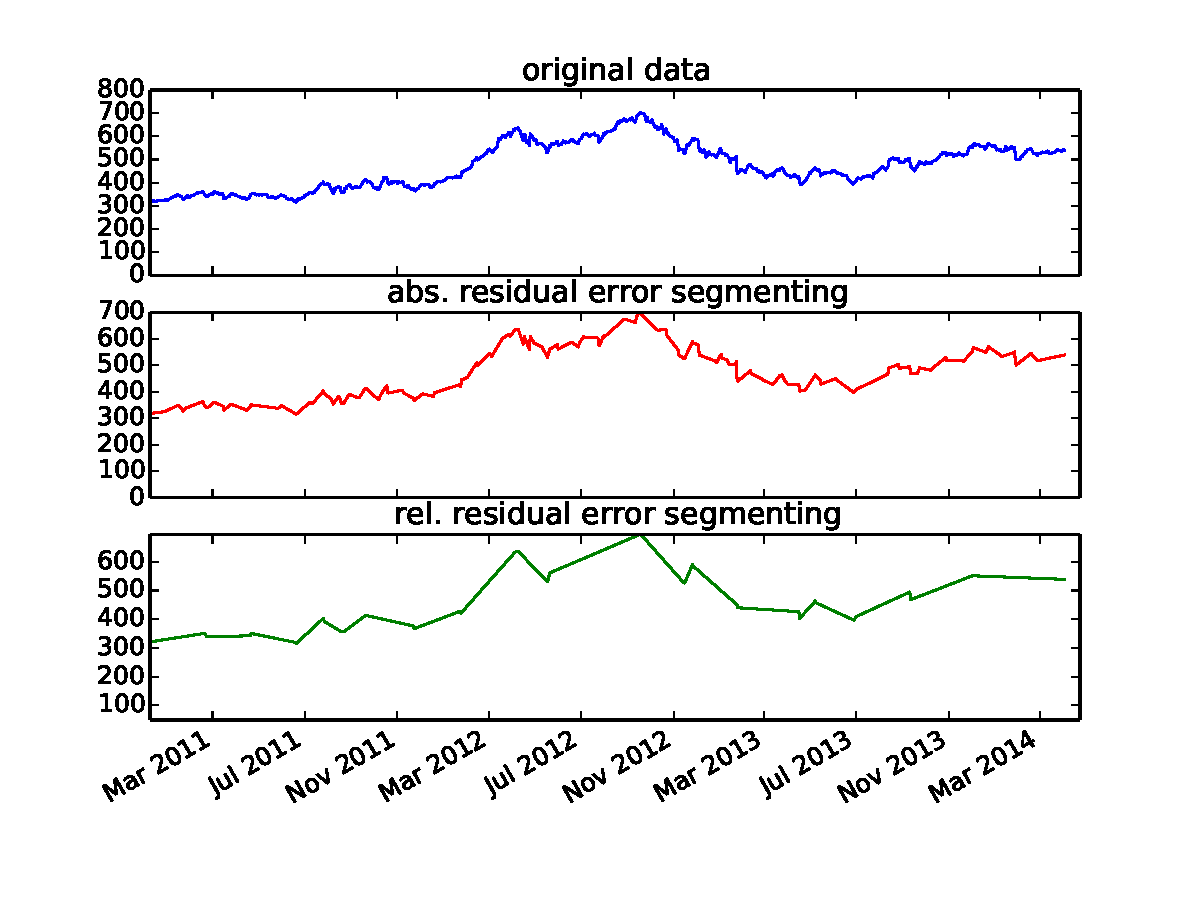
\includegraphics[width=1\textwidth]{aapl-residual-error-comparison.pdf}
\end{center}
\caption{Segmenting error comparison, price of AAPL \label{residuecomp}}
\end{figure}

We stop the segmentation process either when the average length of segments reach a preset amount or the error exceeds a max limit. In our tests, an average segment length (number of original data points merged into a segment) of 20 can reduce the total number of data points from 16000 to about 2000. 

\section{Feature extraction and t-SNE embedding}
Given the segmented time series, we now extract fixed length windows $Ts[i:i+L]$ from the segmented data. Notice that due to the segmenting, we are actually extracting varying length windows of the original data. And so we will obtain a total of len($Ts$)$-L+1$ samples, which we will term a \textit{window}, as our data points for feature extraction. 

First, we borrowed a set of features developed in \cite{Guo07recognizingstock}, for each window of length $L$, we produce the following $L+1$ features:
\begin{align}
f_1 &= \left\{ \begin{array}{rl}
 1 &\mbox{ if $y_1-y_0 \geq 0$} \\
  -1 &\mbox{ otherwise}
       \end{array} \right.\\
f_i &= \frac{y_i-y_{i-1}}{y_{i-1}-y_{i-2}}, \; i=2,\ldots, L,\\
f_{L+1} &= \frac{y_L-y_1}{|y_2-y_1|}.
\end{align}
These features are meant to capture some of the trend characteristics of chart patterns. (1) Indicates the initial direction of the trend, (2) describe the proportions between price movements in each segment of the window, (3) reflects a patterns breaking point. 

We extracted these features on the segmented versions of the daily prices of S\&P500 index, NASDAQ index, Apple, Coke Cola and Exxon Mobile stretching back as far as the 1960's with approximately 10000 data points each, which after segmenting using average segment lengths of 10, 20 and 30 yielded around 2000 to 800 windows. We then fed such data matrices to a binary implementation of the t-distributed Stochastic Neighbour Embedding algorithm. We found that increasing average segment lengths too much resulted in too much smoothing of the data sparser clustering \ref{fig:kosparseclu}.
\begin{figure}[h]
\begin{center}
\begin{subfigure}[b]{0.49\textwidth}
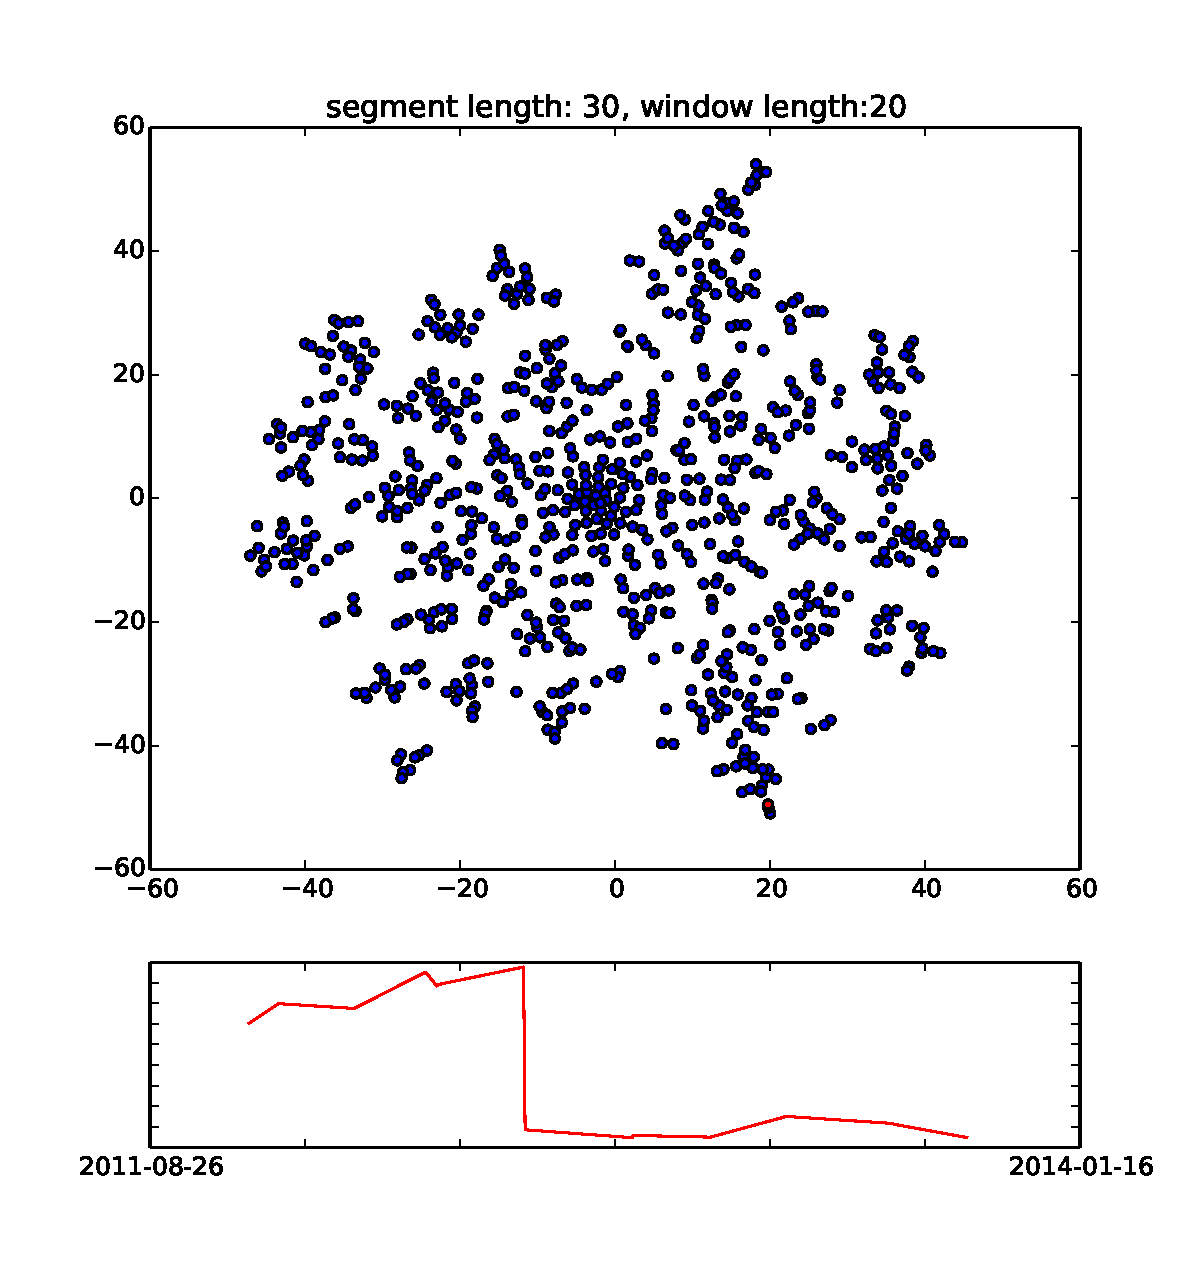
\includegraphics[width=1\textwidth]{ko-30-20-nopattern1.pdf}
                \caption{sparser clusters}
                \label{fig:kosparseclu}
        \end{subfigure}
        \begin{subfigure}[b]{0.49\textwidth}
        		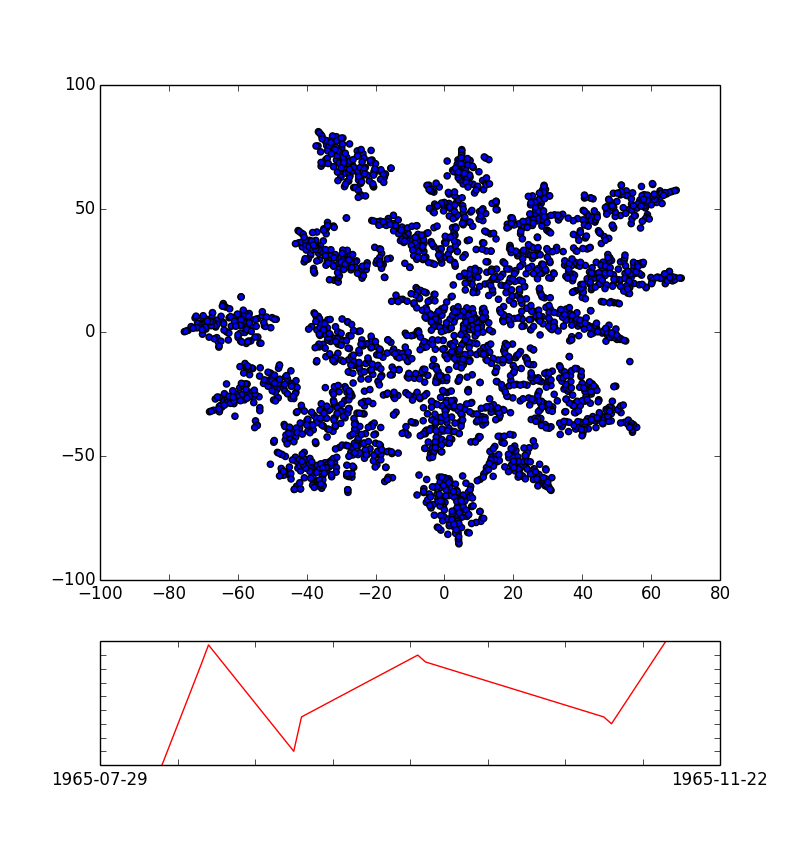
\includegraphics[width=1\textwidth]{ko-10-10-scatter.png}
                \caption{more pronounced clustering}
                \label{fig:ko1010}
        \end{subfigure}
\end{center}
\caption{t-SNE embedding of segmented KO time series using borrowed features.}
\end{figure}
In general, we noticed that while there were noticeable intrinsic clusters found in the 2D embedding using the borrowed feature set, the groupings did not actually capture recognizable patterns used in technical analysis. We hypothesized that the poor performance of these feature sets under t-SNE was due to the fact that each dimension of the feature only depended on a small component of the potential pattern. While the features seemed to have worked with a Self-Organizing Map neural network in \cite{Guo07recognizingstock}, t-SNE is more sensitive to the shape of the manifold in the feature space; that is, similar patterns with only a few differing segments resulted in very dissimilar positions in feature space because each segment essentially resided in an orthogonal dimension.

\subsection{Autocorrelation Features}
With this observation, we developed a new set of features based on a lag-1 autocorrelation of the fixed length windows, hoping to have each feature reflect information about the whole window rather than just single segments. The 2D embedding under these features showed very good intrinsic clustering \ref{fig:aapl-clustered}. Although the grouping is basic, each cluster starting from the top left going in a clockwise fashion represents patterns with rising trend (bullish), downward reversal, decreasing trends (bearish) and upward reversal. This grouping makes sense as the autocorrelation measures exactly this type of temporal dependence in a time series.
\begin{figure}[h]
\begin{center}
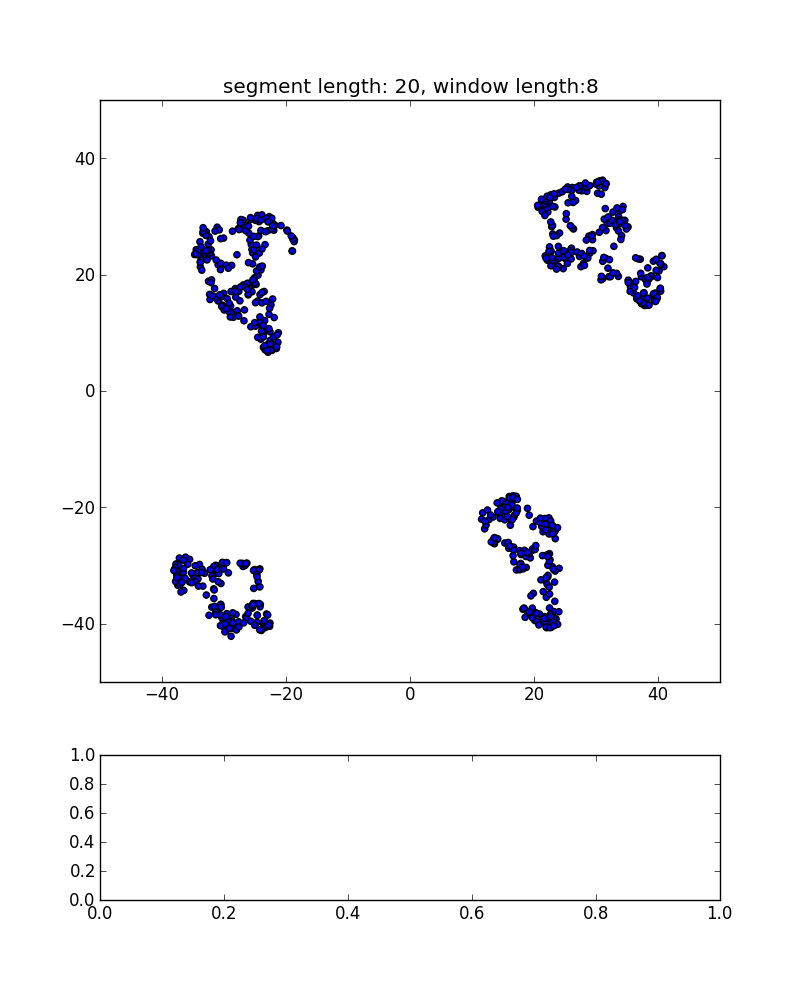
\includegraphics[width=1\textwidth]{aapl-clustered.png}
\end{center}
\caption{t-SNE embedding of autocorrelation features. in ccw order bullish trend, downward reversal, bearish trend and upward reversal\label{fig:aapl-clustered}}
\end{figure}


\section{Conclusion}
While we've found a set of features that loosely categorizes the four basic types of technical patterns: bullish trend, bearish trend, bullish reversal and bearish reversal, these features do not yet capture enough information to accurately describe specific chart patterns. Future improvements we can consider will try to include information about the amount of price movements in a pattern. For example, an appropriately normalized sum of absolute segment lengths feature. We also have not developed high enough dimensional features to really have any crowding problem \cite{Hinton08tsne} that t-SNE is designed to solve. Simply increasing the window length did not improve results, because excessively long windows just add noise to pattern identification. Besides the features themselves, we noticed that there are also scaling issues when plotting the fixed length windows caused by the large price changes over the course of 50+ years that made manual identification of patterns more difficult. This issue can potentially be addressed by using price data from smaller time scales. Finally, we noticed that features developed this way may not necessarily perform equally under other classification or clustering algorithms.
\begin{figure}[h]
\begin{center}
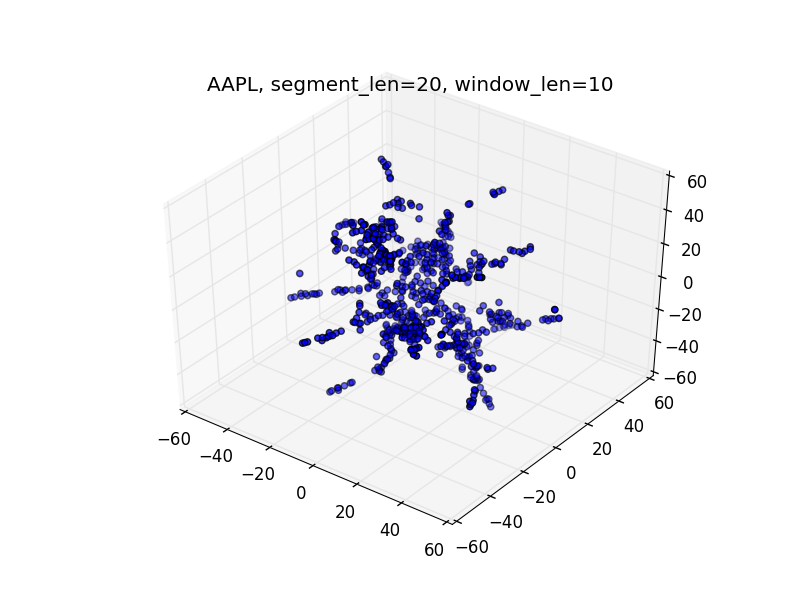
\includegraphics[width=1\textwidth]{aapl-3d-2.png}
\end{center}
\caption{SURPRISE! and here's useless embedding in 3D, AAPL avg. segment length 20, window length 10}
\end{figure}

\bibliographystyle{plain}
\bibliography{biblio}

\end{document}
